\apendice{Especificación de diseño}

\section{Introducción}\label{introducción-diseño}

En este apéndice se abordarán los aspectos relacionados con el diseño de tratamiento de datos, el diseño de procesos y el diseño arquitectónico, seguidos a lo largo del desarrollo de este proyecto

\section{Diseño de datos}\label{diseño-de-datos}

En esta sección, se describen las estructuras de datos utilizadas en la aplicación. Los datos de entrada son imágenes que se procesan mediante una serie de scripts. Las librerías de MATLAB gestionan operaciones específicas como la manipulación de imágenes y el análisis de datos. Las variables globales se utilizan para almacenar información clave, como parámetros de configuración y resultados intermedios.

\subsection{Convección de nombres de imágenes}\label{convección-de-nombres-de-imágenes}

A continuación se detallan las distintas convenciones de nombres de las imágenes tanto de las proporcionadas por la aplicación como de las imágenes resultado.

\subsubsection{Imágenes proporcionadas por la aplicación}\label{imágenes-proporcionadas-por-la-aplicación}

Las imágenes proporcionadas por el sistema están nombrados siguiendo una convención específica que facilita la comprensión rápida del contenido y las características de cada imagen. Cada imagen contiene información relevante como el número de piezas metálicas, si las piezas son iguales o distintas, el número de focos de luz utilizados, el material de las piezas (como aluminio, acero o hierro) y la técnica de formado aplicada (como troquelado o lisa). Estos elementos se codifican en el nombre del archivo utilizando abreviaturas, lo que permite identificar rápidamente las características de cada imagen sin necesidad de abrir el archivo.

La convención de nombres de archivos sigue un formato preestablecido: `<Número de Piezas>\_<Forma de las Piezas>\_<Número de Focos>\_<Material>\_<Técnica>.jpg'. Por ejemplo, el archivo `3\_DIS\_1\_ALU \_TRO.jpg' indica que contiene una imagen con tres piezas metálicas distintas, iluminadas por un solo foco de luz, hechas de aluminio y formadas mediante troquelado. De manera similar, el archivo 2\_IGU\_2\_ACE\_LIS.jpg sugiere que la imagen contiene dos piezas metálicas iguales, iluminadas por dos focos de luz, hechas de acero y formadas con una técnica lisa. Esta metodología de nomenclatura asegura una identificación rápida y eficiente del contenido y las características principales de cada imagen, facilitando el análisis y la organización de los archivos.

\subsubsection{Imágenes resultado}\label{imágenes-resultado}

Las imágenes de solución tienen los nombres formateados de la siguiente manera:
\begin{itemize}
    \item fecha\_1\_\_nombre\_\_invariante.extensión
    \item fecha\_2\_\_nombre\_\_Original\_agrupamiento\_numeroDeCentros\_c\_ acierto\%.extensión
    \item fecha\_3\_\_nombre\_\_invariante\_agrupamiento\_numeroDeCentros\_c \_acierto\%.extensión
\end{itemize}

Estos nombres reflejan la fecha de ejecución, el nombre de la imagen, el algoritmo utilizado, el número de centros y el porcentaje de acierto, lo que permite una organización clara y detallada de las imágenes.

Estos son los mismos nombres que acepta la memoria caché, por lo que se pueden copiar y pegar imágenes en la memoria caché para agilizar la ejecución. Al mantener la coherencia en el formato de los nombres de los archivos, se facilita su uso en procesos automatizados y se optimiza el rendimiento del sistema al reducir el tiempo de acceso a las imágenes necesarias durante la ejecución de las tareas.

\section{Diseño procedimental}\label{diseño-procedimental}

En este apartado se recogen los detalles más relevantes respecto a la ejecución de la aplicación desde que el usuario selecciona una imagen a analizar hasta que guarda los resultados.

\begin{figure}[!h]
    \centering
    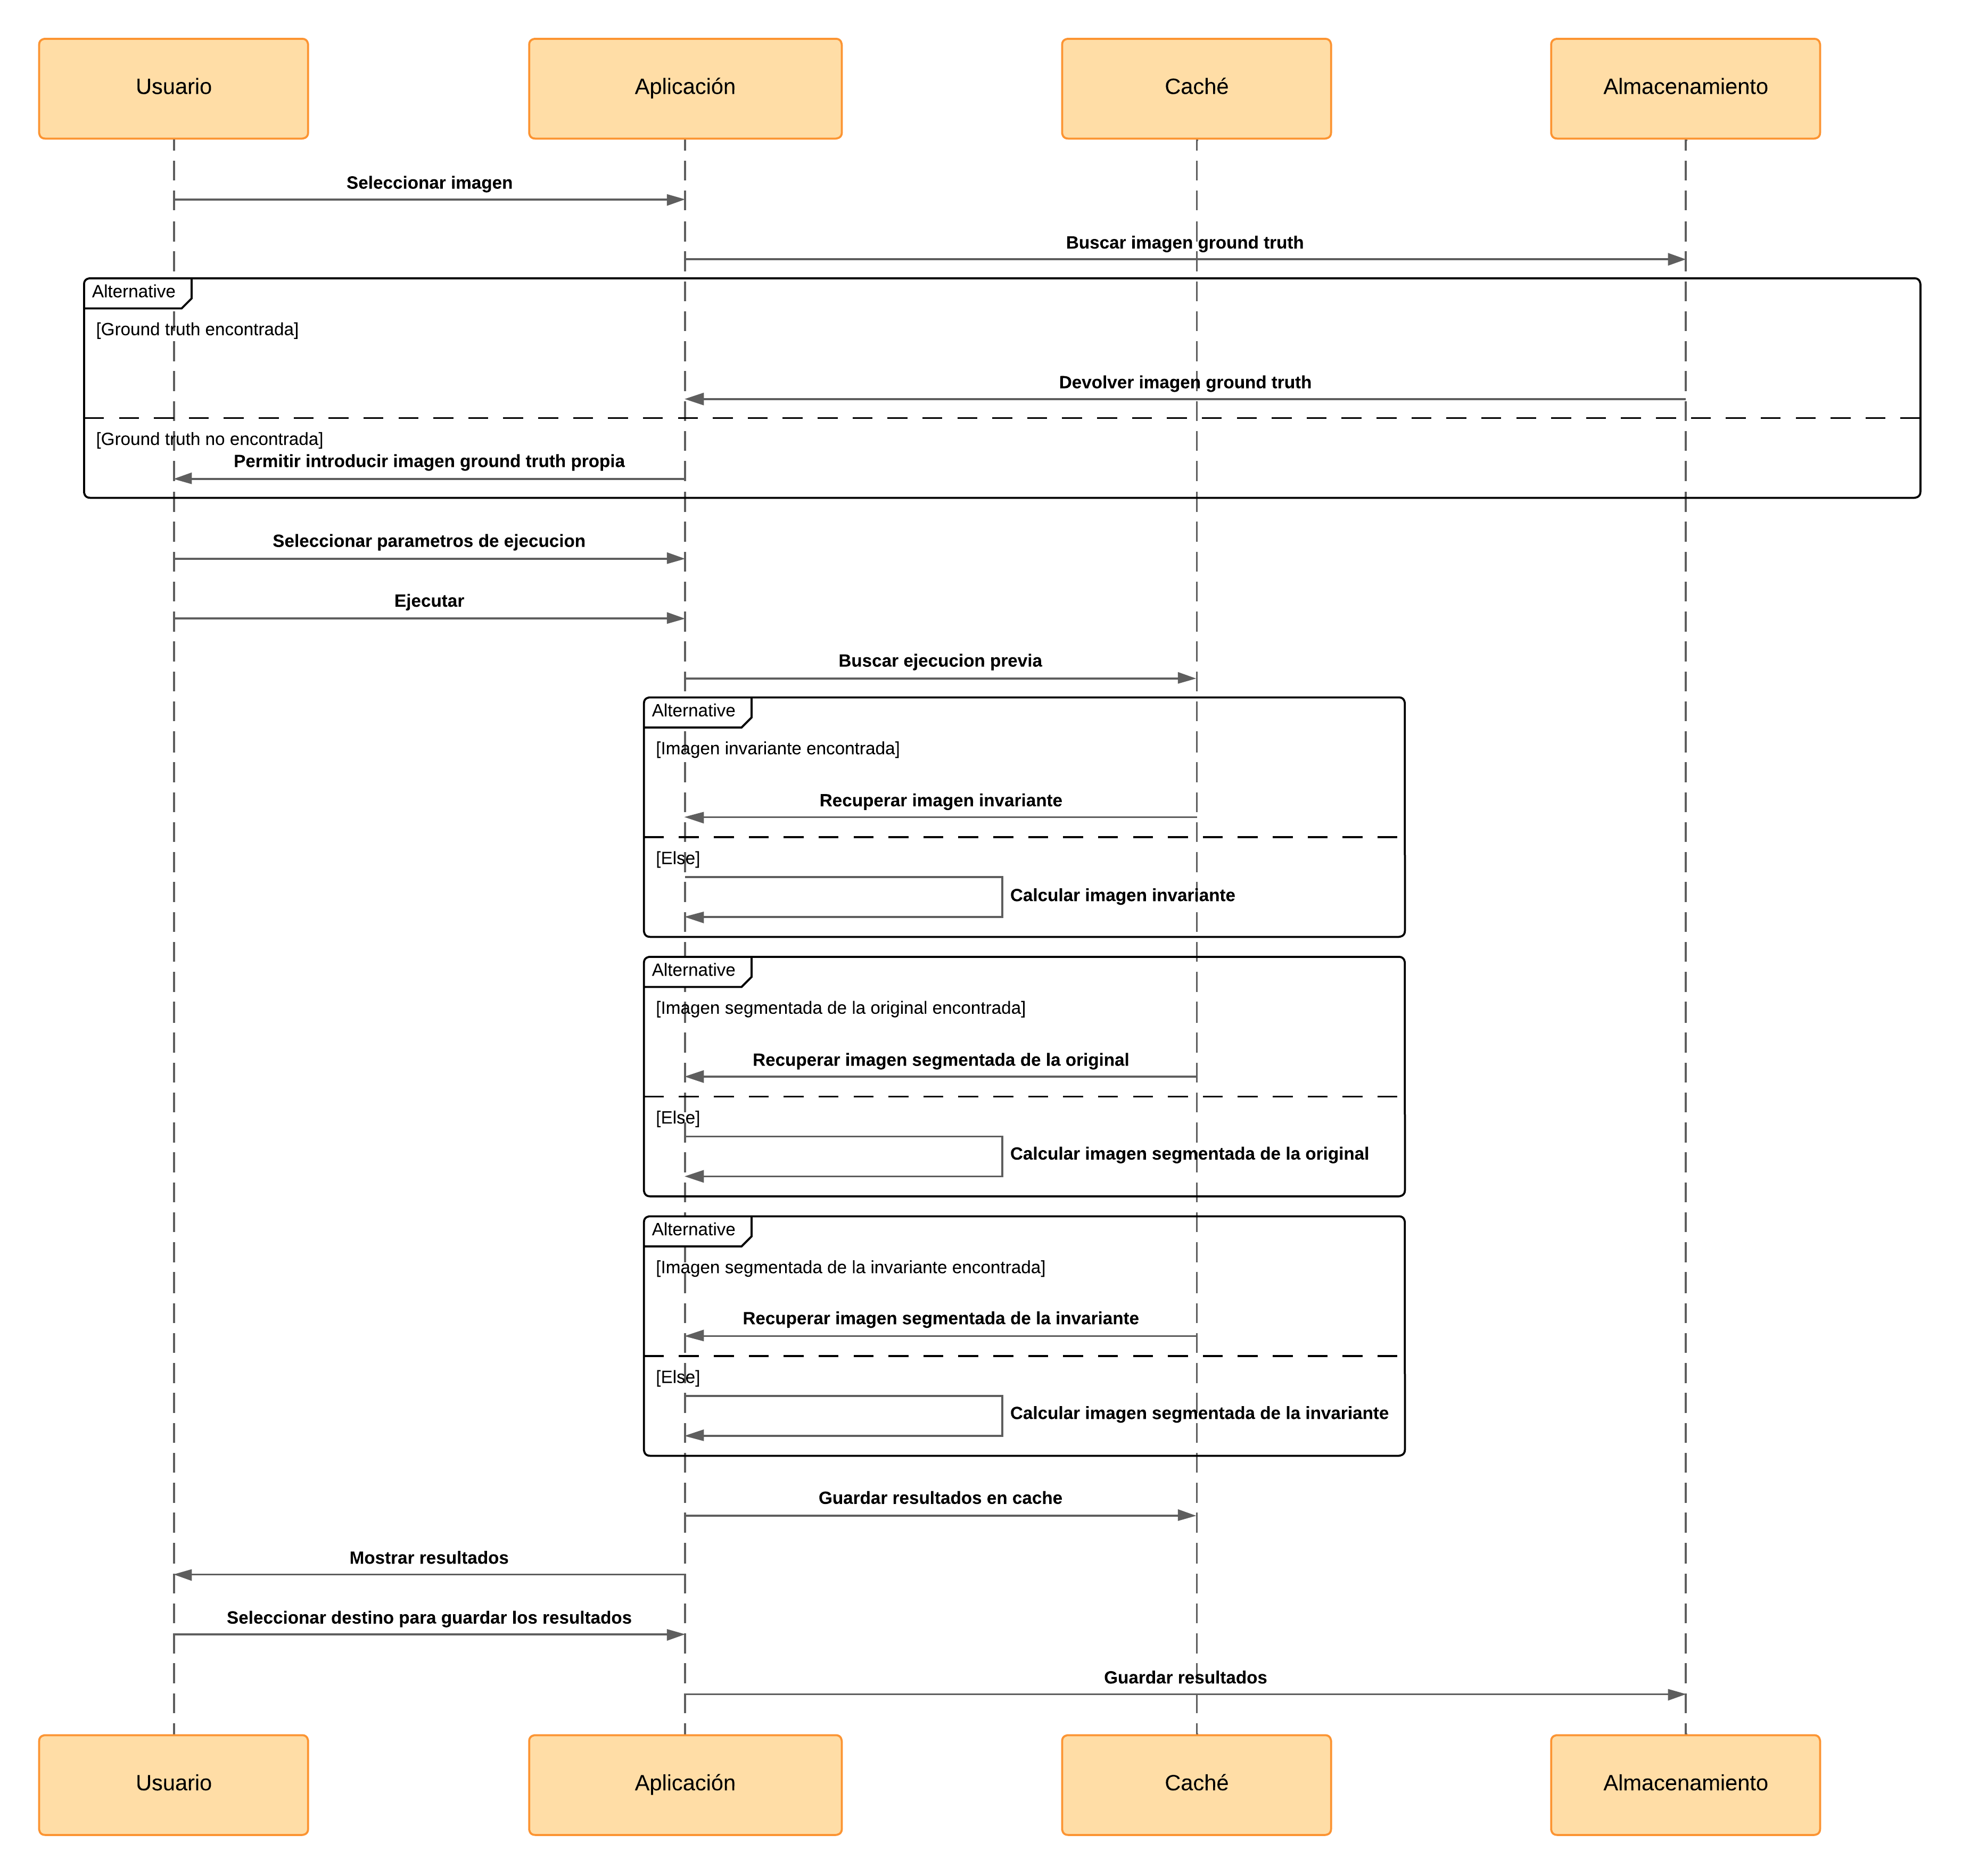
\includegraphics[width=1.1\textwidth]{Diagrama_de_secuencia}
    \caption{Diagrama de secuencia correspondiente al caso de uso 01 gestión de la trasformación de invariante de iluminación.}\label{fig:Diagrama_de_secuencia}
\end{figure}

El proceso se inicia cuando el usuario selecciona una imagen que contenga piezas metálicas. La imagen se carga y se preprocesa eliminando el canal alpha. A continuación se le aplica sobre la imagen el algoritmo de transformación invariante seleccionado. Después se aplica sobre la imagen original y sobre la imagen invariante el método de agrupamiento. Posteriormente, en el caso de que tenga imagen ground truth, se calcula el porcentaje de acierto de las segmentaciones. Finalmente, los resultados se presentan al usuario, quien tiene la opción de guardarlos.

\imagen{Diagrama_de_flujo}{Diagrama de flujo detallado del procesamiento de datos en la aplicación.}

En la figura \ref{fig:Diagrama_de_flujo} se muestra de un diagrama de flujo con los pasos a seguir desde que el usuario selecciona una imagen hasta que este la guarda.

\section{Diseño arquitectónico}\label{diseño-arquitectónico}

La arquitectura de la aplicación está basada en una serie de módulos interconectados que utilizan funciones específicas para implementar los casos de uso. A continuación se presentan los componentes principales:

\begin{itemize}
    \item \textbf{Interfaz de usuario:} permite la carga de imágenes, la selección de transformación invariante, la selección de número de centros, la selección de algoritmo de agrupamiento y la visualización de resultados ente otras cosas.
    \item \textbf{Módulo de procesamiento:} son todas aquellas funciones que la aplicación ejecuta de forma opaca al usuario que hacen uso de los scripts para obtener los resultados.
    \item \textbf{Bibliotecas de MATLAB:} conjunto de funciones predefinidas utilizadas para operaciones específicas de manipulación de datos y análisis de imágenes.
    \item \textbf{Sistema de almacenamiento:} hay de tres tipos:
        \begin{itemize}
            \item `/data' que guarda las imágenes de prueba y su correspondiente imagen ground truth.
            \item `/cache' que se encarga de almacenar los resultados de todos las anteriores ejecuciones exceptuando el caso de que el usuario lo desee eliminar.
            \item `/results' que es la ruta donde se almacenan por defecto las imágenes que el usuario desea guardar.
        \end{itemize}
\end{itemize}

\begin{figure}[!h]
    \centering
    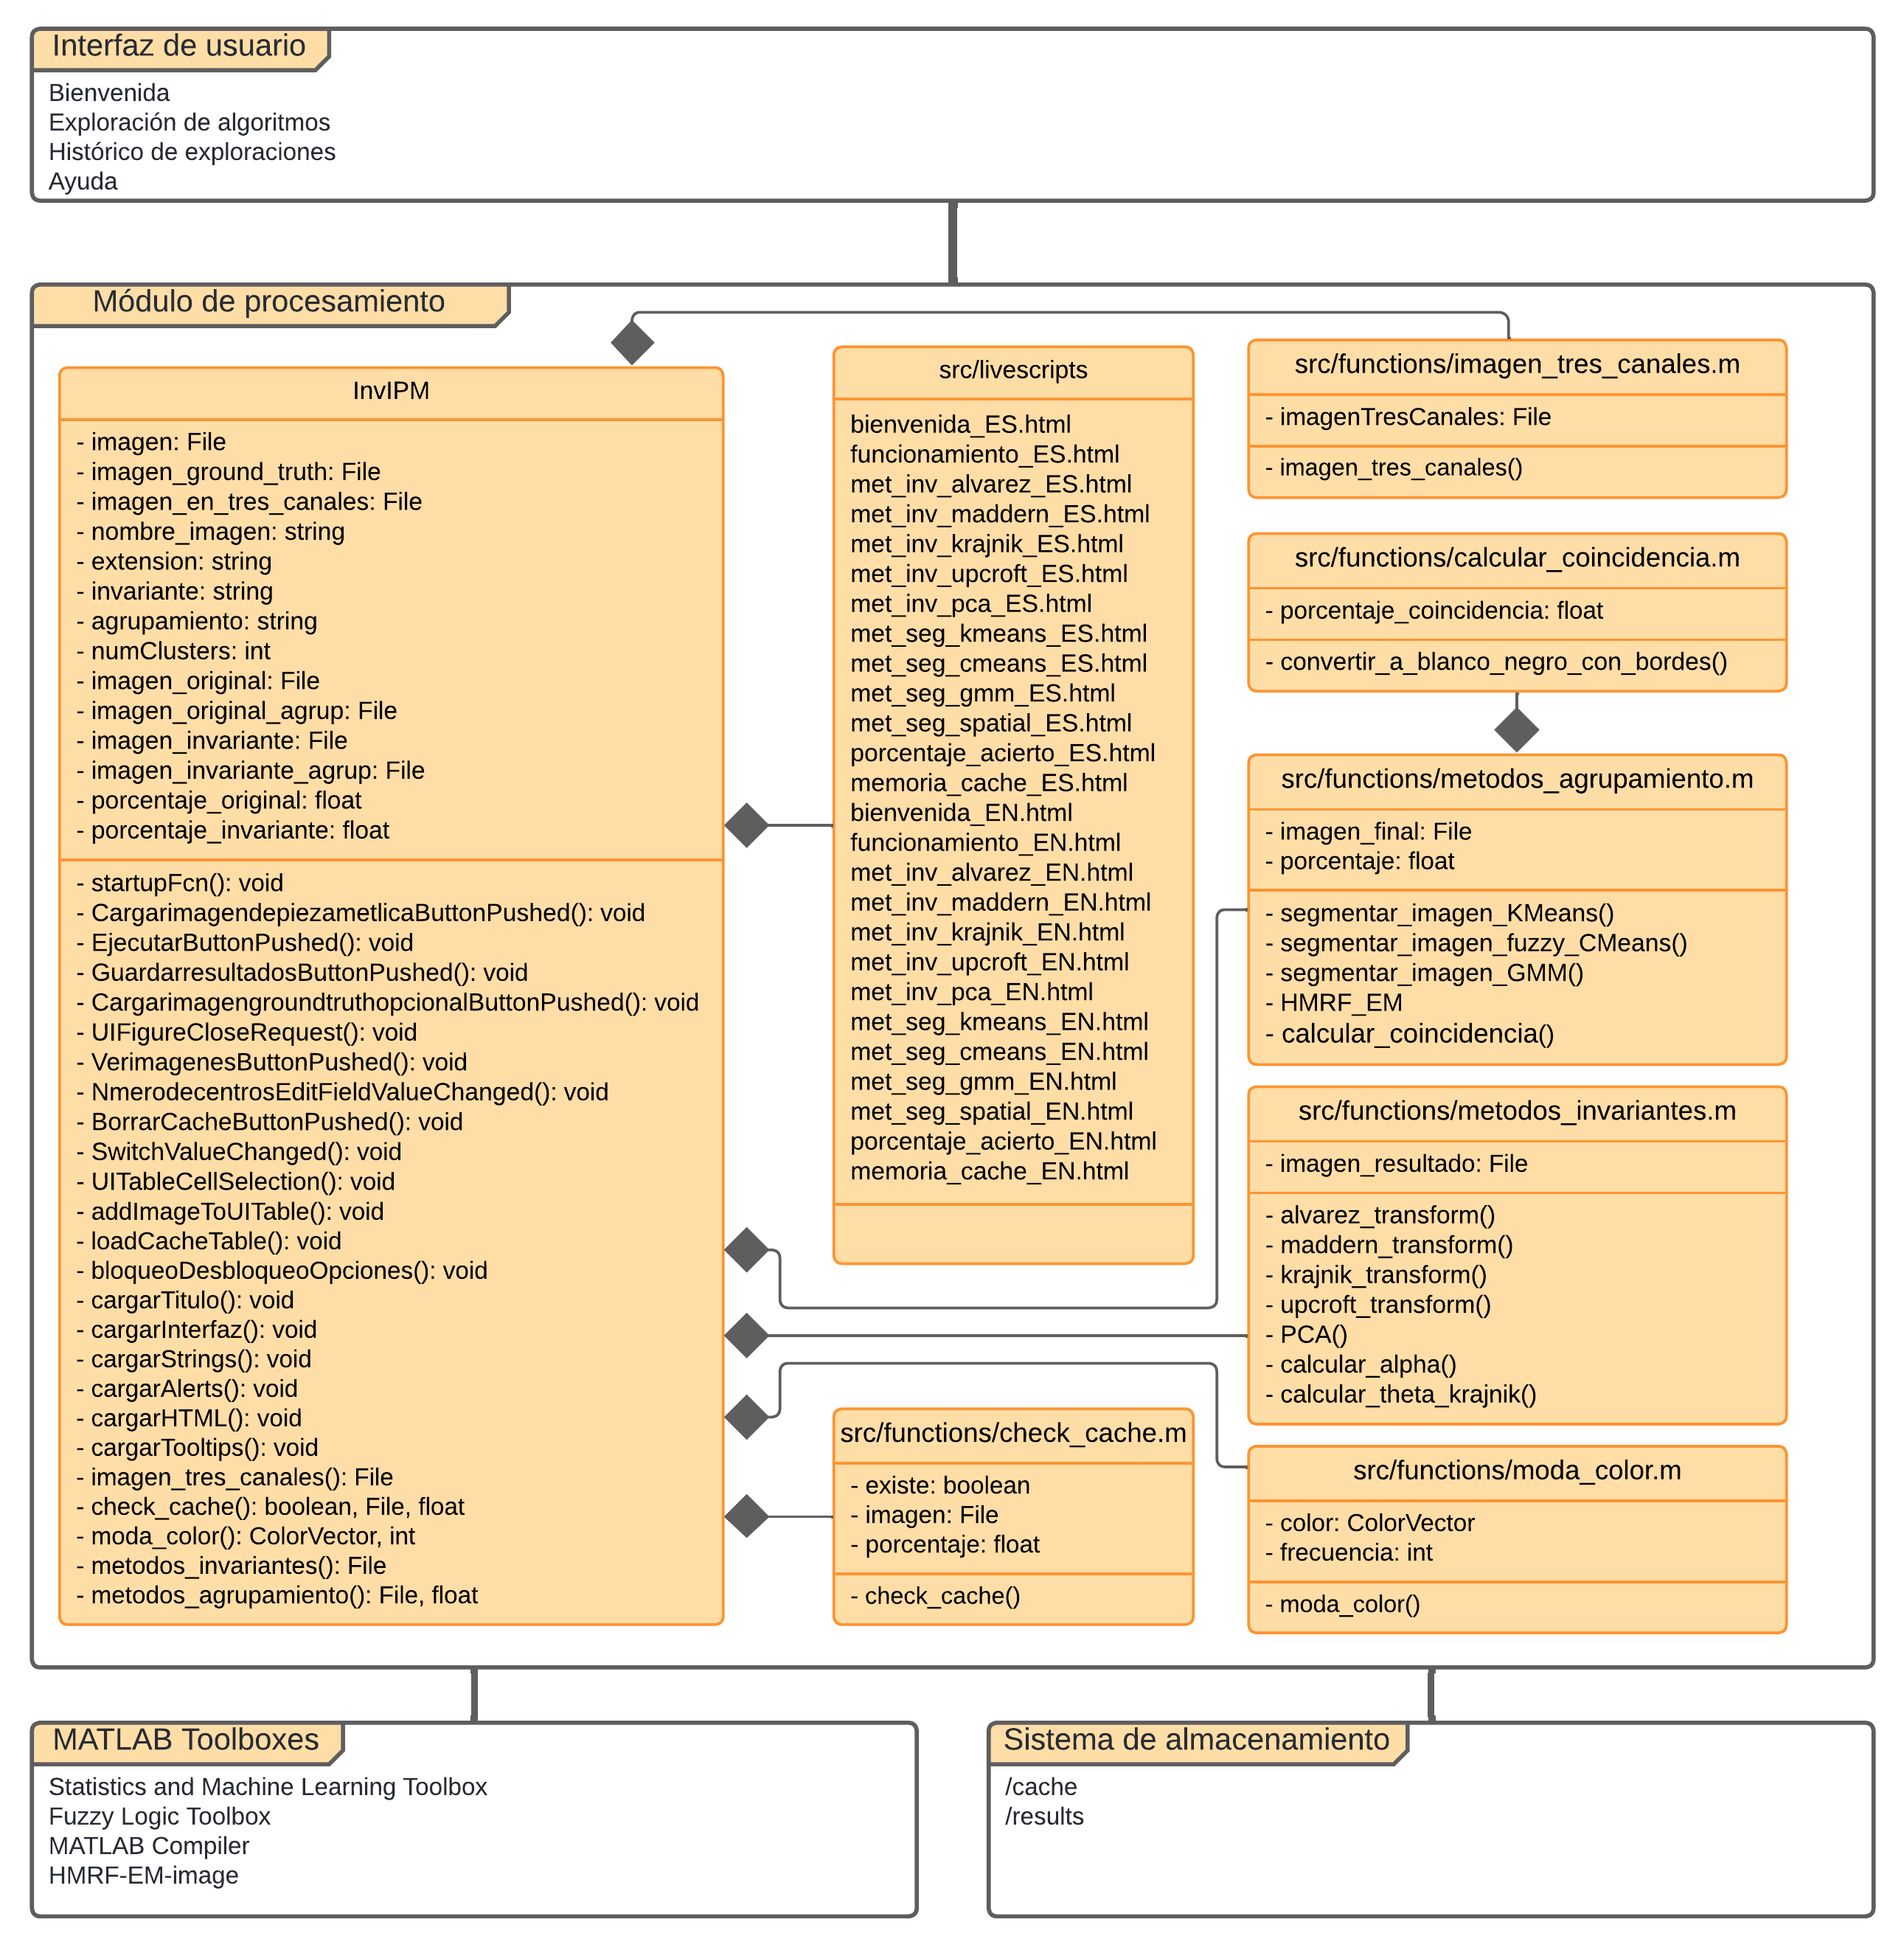
\includegraphics[width=1.1\textwidth]{Diagrama_de_componentes}
    \caption{Diagrama de componentes mostrando la interacción entre los distintos módulos de la aplicación.}\label{fig:Diagrama_de_componentes}
\end{figure}

En la figura \ref{fig:Diagrama_de_componentes} se muestra la interacción que tienen los distintos componentes de la aplicación.
